\chapter{Test}
\label{chap:test}

\section{Test ``Analisi assistita''}
\noindent Per effettuare i test dell’estensione sono stati utilizzati alcuni siti realizzati per l’ultima edizione del concorso \textit{Accattivante Accessibile}.\
I test hanno preso in considerazione gli errori individuati da TV insieme a quelli segnalati dalla docente referente e sono stati messi a confronto con gli errori rilevati da \textit{SviluppAbile}.
Infine, ho confrontato i risultati elaborando un resoconto per ciascun sito analizzato e, successivamente, ho applicato la metrica F1-score per ottenere un report oggettivo.

\subsection{F1-score}
\noindent La F\textsubscript{1}-score è una metrica utilizzata per valutare modelli di classificazione, sia binari che multi‐classe. Essa combina in un unico valore la \textit{precision} (quanto le predizioni positive sono corrette) e il \textit{recall} (quanti casi positivi reali vengono identificati), calcolati come:

\[
\text{Precision} = \frac{TP}{TP + FP}, 
\qquad
\text{Recall} = \frac{TP}{TP + FN}
\]

\vspace{0.5cm}
\noindent L’F\textsubscript{1}-score è definita come la media armonica di tali valori:

\[
F_{1} = 2 \cdot \frac{\text{Precision} \cdot \text{Recall}}{\text{Precision} + \text{Recall}}
 = \frac{2 \cdot TP}{2 \cdot TP + FP + FN}
\]
\vspace{0.1cm}

\noindent Questo significa che nel calcolo verranno utilizzati i tre dati rilevati nel presente lavoro:
"errori trovati" come \(TP\) (veri positivi), "errori non trovati" come \(FN\) (falsi negativi), e \(FP\) (falsi positivi).
In questo modo, l’F\textsubscript{1}-score riflette in modo equilibrato sia la capacità di individuare correttamente errori reali, sia il controllo sui falsi allarmi.\\

\noindent L’F\textsubscript{1}-score assume valori compresi tra 0 e 1. Il valore minimo, \(0\), indica prestazioni pessime (almeno una delle due metriche è nulla), mentre il valore massimo, \(1\), corrisponde a prestazioni perfette (precisione e recall entrambi pari a 1).\\
Valori prossimi a 1 indicano quindi un buon funzionamento del sistema, mentre valori vicini a 0 segnalano performance insoddisfacenti.


% SUDOKU WORLD
\subsection{Sito web: SudokuWorld}
\noindent Di seguito vengono riportati alcuni dei test effettuati sul sito \href{https://caa.studenti.math.unipd.it/amonaco/Sudokuworld/pages/home.php}{SudokuWorld}.

\subsubsection{Total Validator}
\begin{figure}[H]
    \centering
    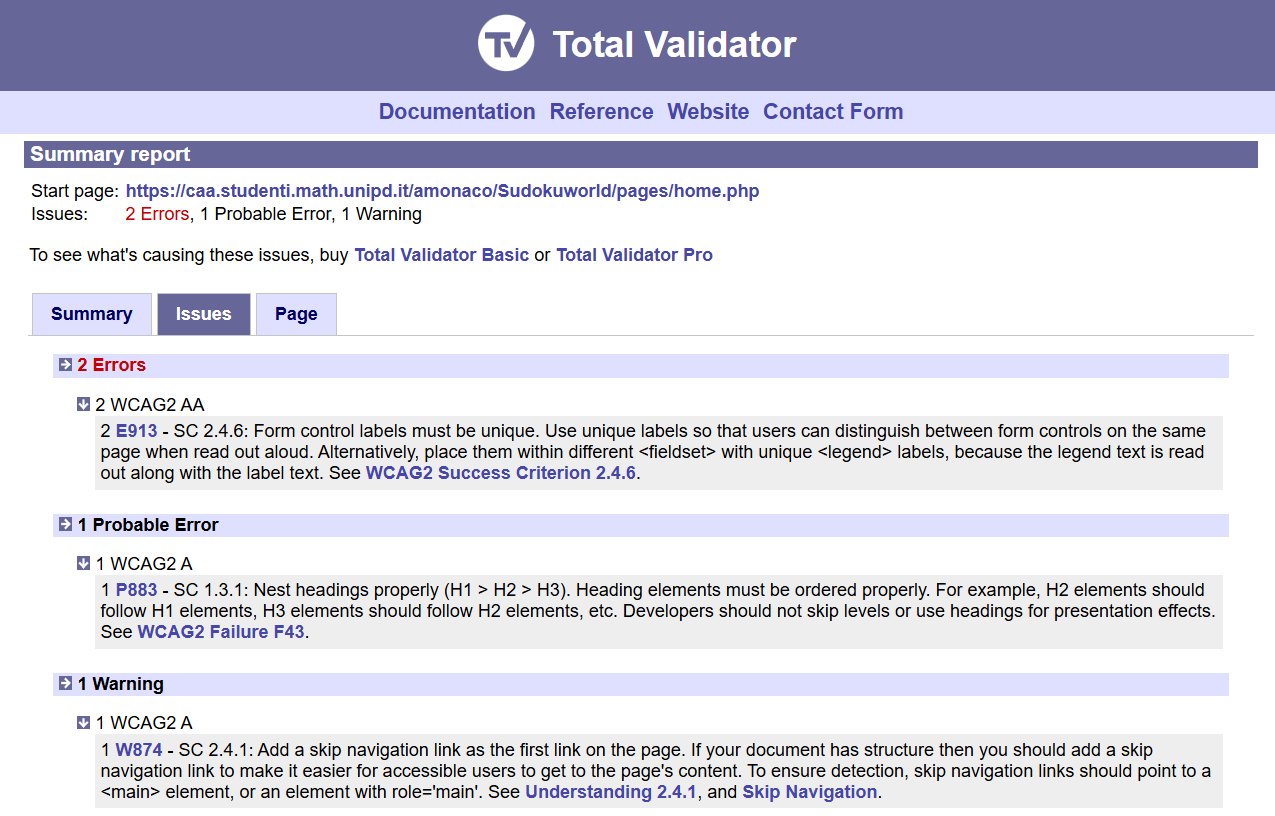
\includegraphics[width=0.7\linewidth, alt={Screenshot dell'analisi di Total Validator sul sito web SudokuWorld}]{img/TV_sudoku.png}
    \caption{Analisi di Total Validator sul sito web \textit{SudokuWorld}}\label{fig:TV_sudoku}
\end{figure}

\noindent Come visibile nella figura \ref{fig:TV_sudoku} è possibile vedere che lo strumento \acrshort{tv} trova ben 15 errori di accessibilità.\\
Gli errori principali sono: 
\begin{itemize}
    \item E913 - SC 2.4.6: Le etichette dei controlli dei \glslink{formg}{form} devono essere univoche. Utilizzare etichette univoche consente agli utenti di distinguere i vari controlli presenti sulla stessa pagina quando vengono letti da uno screen reader. In alternativa, è possibile inserirli all’interno di diversi <fieldset> con <legend> univoci, poiché il testo del <legend> viene letto insieme all’etichetta del controllo. Vedi WCAG2 Success Criterion 2.4.6.
    \item P883 - SC 1.3.1: Nidificare correttamente le intestazioni (H1 > H2 > H3). Gli elementi di intestazione devono essere ordinati in modo gerarchico. Ad esempio, un elemento H2 dovrebbe seguire un H1, un H3 dovrebbe seguire un H2, e così via. Gli sviluppatori non devono saltare livelli né utilizzare le intestazioni solo per scopi di presentazione. Vedi WCAG2 Failure F43.
\end{itemize}

\subsubsection{Lighthouse}
\noindent Il report generato dallo strumento Lighthouse ha restituito un punteggio di 100/100 nella sezione Accessibility, indicando che, secondo le metriche automatiche adottate, non sono stati rilevati errori o problematiche di conformità (vedi figura \ref{fig:Lighthouse_sudoku}).
\begin{figure}[H]
    \centering
    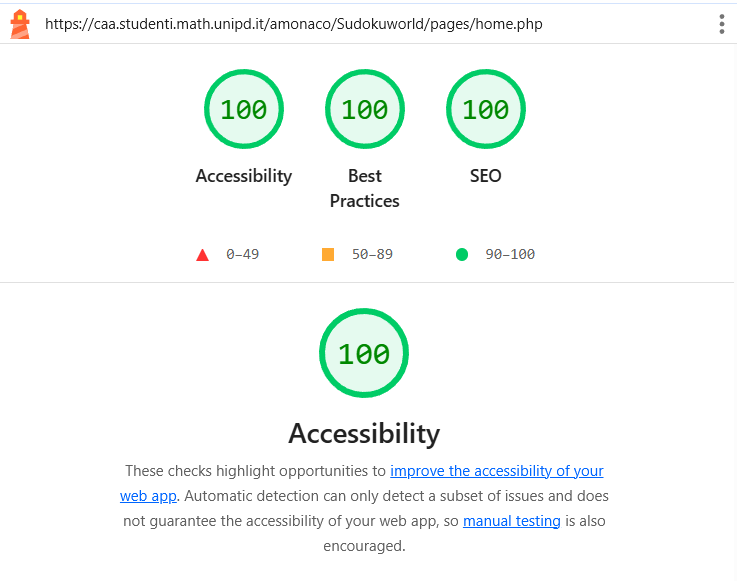
\includegraphics[width=0.6\linewidth, alt={Screenshot dell'analisi di Lighthouse sul sito web SudokuWorld}]{img/Lighthouse_sudoku.png}
    \caption{Analisi di Lighthouse sul sito web \textit{SudokuWorld}}\label{fig:Lighthouse_sudoku}
\end{figure}

\subsubsection{SviluppAbile}

\subsubsection{Resoconto finale}
\noindent Nella tabella \ref{tab:sudokuWorld} viene fatto un riassunto/resoconto degli errori trovati

\begin{footnotesize}
\begin{longtable}[c]{|C{2.85cm}|C{8cm}|C{2.85cm}|}
\caption{Tabella riassuntiva analisi \textit{SudokuWorld} tramite \textit{SviluppAbile}}
\label{tab:sudokuWorld}\\
\hline
\textbf{Errori trovati} & \textbf{Errori non trovati} & \textbf{Falsi positivi}\\
\hline
\endfirsthead
\multicolumn{3}{c}%
{{\bfseries Tabella \thetable\ -- continua dalla pagina precedente}} \\
\hline
\textbf{Errori trovati} & \textbf{Errori non trovati} & \textbf{Falsi positivi}\\
\hline
\endhead
\hline
\multicolumn{3}{r}{{ -- continua nella pagina successiva}} \\
\endfoot
\hline
\endlastfoot
\textbf{RD-01} & xx & UC xx\\
\hline
\textbf{RD-02} & xx & UC xx\\
\hline
\end{longtable}
\end{footnotesize}


% DOLCE RISVEGLIO
\subsection{Sito web: Dolce Risveglio}
\noindent Di seguito vengono riportati alcuni dei test effettuati sul sito \href{https://caa.studenti.math.unipd.it/gchecchi/}{DolceRisveglio}.

\subsubsection{Total Validator}
\begin{figure}[H]
    \centering
    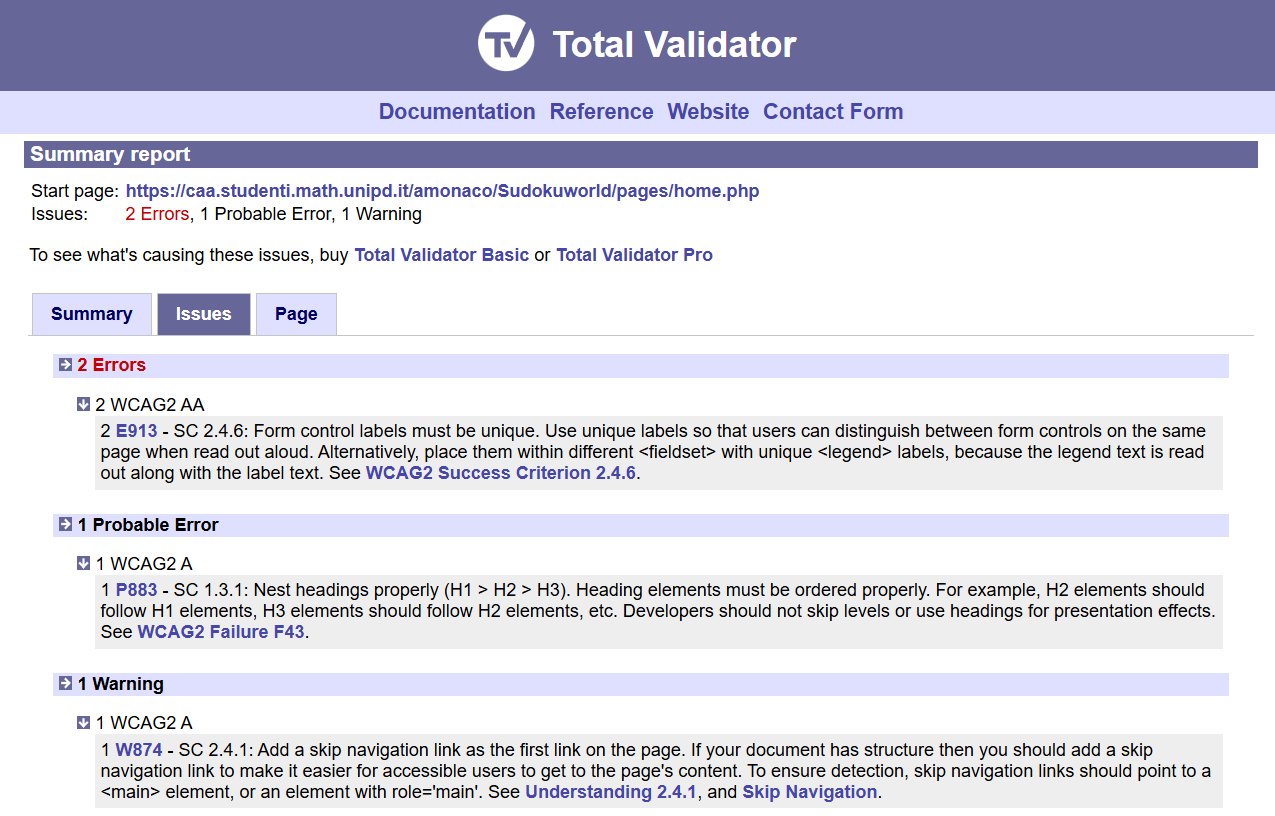
\includegraphics[width=0.8\linewidth, alt={Screenshot dell'analisi di Total Validator sul sito web Dolce Risveglio}]{img/TV_sudoku.png}
    \caption{Analisi di Total Validator sul sito web \textit{Dolce Risveglio}}\label{fig:TV_sudoku}
\end{figure}

\noindent Come visibile nella figura \ref{fig:TV_sudoku} è possibile vedere che lo strumento \acrshort{tv} trova ben 15 errori di accessibilità.\\
Gli errori principali sono: 
\begin{itemize}
    \item E913 - SC 2.4.6: Le etichette dei controlli dei \glslink{formg}{form} devono essere univoche. Utilizzare etichette univoche consente agli utenti di distinguere i vari controlli presenti sulla stessa pagina quando vengono letti da uno screen reader. In alternativa, è possibile inserirli all’interno di diversi <fieldset> con <legend> univoci, poiché il testo del <legend> viene letto insieme all’etichetta del controllo. Vedi WCAG2 Success Criterion 2.4.6.
    \item P883 - SC 1.3.1: Nidificare correttamente le intestazioni (H1 > H2 > H3). Gli elementi di intestazione devono essere ordinati in modo gerarchico. Ad esempio, un elemento H2 dovrebbe seguire un H1, un H3 dovrebbe seguire un H2, e così via. Gli sviluppatori non devono saltare livelli né utilizzare le intestazioni solo per scopi di presentazione. Vedi WCAG2 Failure F43.
\end{itemize}

\subsubsection{Lighthouse}
\noindent Il report generato dallo strumento Lighthouse ha restituito un punteggio di 100/100 nella sezione Accessibility, indicando che, secondo le metriche automatiche adottate, non sono stati rilevati errori o problematiche di conformità (vedi figura \ref{fig:Lighthouse_sudoku}).
\begin{figure}[H]
    \centering
    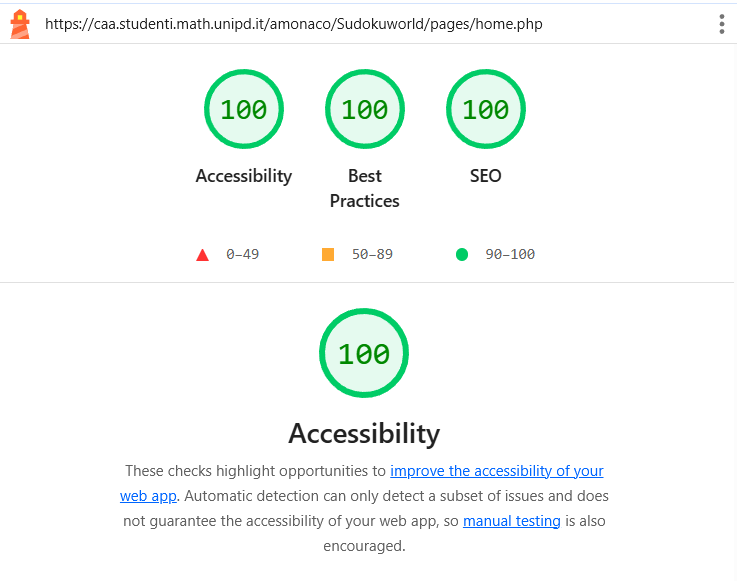
\includegraphics[width=0.6\linewidth, alt={Screenshot dell'analisi di Lighthouse sul sito web SudokuWorld}]{img/Lighthouse_sudoku.png}
    \caption{Analisi di Lighthouse sul sito web \textit{Dolce Risveglio}}\label{fig:Lighthouse_sudoku}
\end{figure}

\subsubsection{SviluppAbile}
\noindent Di seguito vengono riportate alcune domande fatte e risposte ricevute dall'estensione \textit{SviluppAbile}. \newline
\\ \vspace{-0.5cm}
\noindent(pagina home.php)\\
\subsubsection*{\texttt{Il mio codice HTML rispetta le linee guida WCAG?}}
\begin{adjustwidth}{1cm}{1cm}
\noindent {\footnotesize xxx }
\end{adjustwidth}

% E-LIXIRIUM
\subsection{Sito web: E-lixirium}
\noindent Di seguito vengono riportati alcuni dei test effettuati sul sito \href{https://caa.studenti.math.unipd.it/abaldazz/?page=home}{E-lixirium}.

% CORSA IDEALE
\subsection{Sito web: Corsa Ideale}
\noindent Di seguito vengono riportati alcuni dei test effettuati sul sito \href{https://caa.studenti.math.unipd.it/epinarel/}{Corsa Ideale}.

% BOOKOVERFLOW
\subsection{Sito web: BookOverflow}
\noindent Di seguito vengono riportati alcuni dei test effettuati sul sito \href{https://caa.studenti.math.unipd.it/lribon/}{BookOverflow}, sito web vincitore del concorso.
\subsubsection{Total Validator}
\begin{figure}[H]
    \centering
    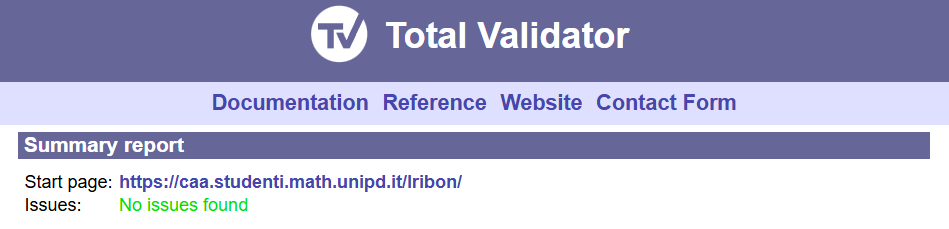
\includegraphics[width=0.8\linewidth, alt={Screenshot dell'analisi di Total Validator sul sito web BookOverflow}]{img/TV_bookoverflow.png}
    \caption{Analisi di Total Validator sul sito web \textit{BookOverflow}}\label{fig:TV_bookoverflow}
\end{figure}

\noindent Come visibile in figura \ref{fig:TV_bookoverflow}, non vi sono errori di accessibilità.

\subsubsection{Lighthouse}
\noindent Il report generato dallo strumento Lighthouse ha restituito un punteggio di 100/100 nella sezione Accessibility, indicando che, secondo le metriche automatiche adottate, non sono stati rilevati errori o problematiche di conformità (vedi figura \ref{fig:Lighthouse_bookoverflow}).
\begin{figure}[H]
    \centering
    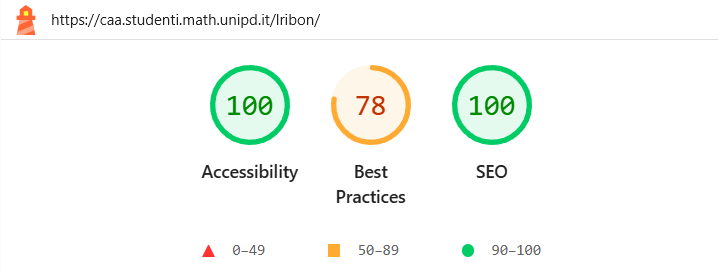
\includegraphics[width=0.6\linewidth, alt={Screenshot dell'analisi di Lighthouse sul sito web BookOverflow}]{img/Lighthouse_bookoverflow.png}
    \caption{Analisi di Lighthouse sul sito web \textit{BookOverflow}}\label{fig:Lighthouse_bookoverflow}
\end{figure}

\subsubsection{SviluppAbile}
\noindent Nella tabella \ref{tab:bookoverflow} vengono riportati i risultati ottenuti utilizzando l'estensione \textit{SviluppAbile}.
\begin{footnotesize}
\begin{longtable}[c]{|C{4.6cm}|C{4.6cm}|C{4.6cm}|}
\caption{Tabella riassuntiva analisi \textit{BookOverflow} tramite \textit{SviluppAbile}}
\label{tab:bookoverflow}\\
\hline
\textbf{Errori trovati} & \textbf{Errori non trovati} & \textbf{Falsi positivi}\\
\hline
\endfirsthead
\multicolumn{3}{c}%
{{\bfseries Tabella \thetable\ -- continua dalla pagina precedente}} \\
\hline
\textbf{Errori trovati} & \textbf{Errori non trovati} & \textbf{Falsi positivi}\\
\hline
\endhead
\hline
\multicolumn{3}{r}{{ -- continua nella pagina successiva}} \\
\endfoot
\hline
\endlastfoot
 & 
\begin{itemize}
    \item Contrasto insufficiente link visitati/non
\end{itemize}
 & \begin{itemize}
    \item Tabindex non adeguato
\end{itemize}\\
\hhline{|=|=|=|} 
0 & 1 & 1 \\
\end{longtable}
\end{footnotesize}

\noindent L'F\textsubscript{1}-score calcolato è $F_{1}=0$, valore che indica prestazioni non soddisfacenti in questo caso specifico. 
Ciò evidenzia la necessità di ulteriori miglioramenti nell’identificazione degli errori, soprattutto per quanto riguarda i falsi positivi.

% LUZZAUTO
\subsection{Sito web: LuzzAuto}
\noindent Di seguito vengono riportati alcuni dei test effettuati sul sito \href{https://caa.studenti.math.unipd.it/eartusi/index.php}{LuzzAuto}.
\subsubsection{Total Validator}
\begin{figure}[H]
    \centering
    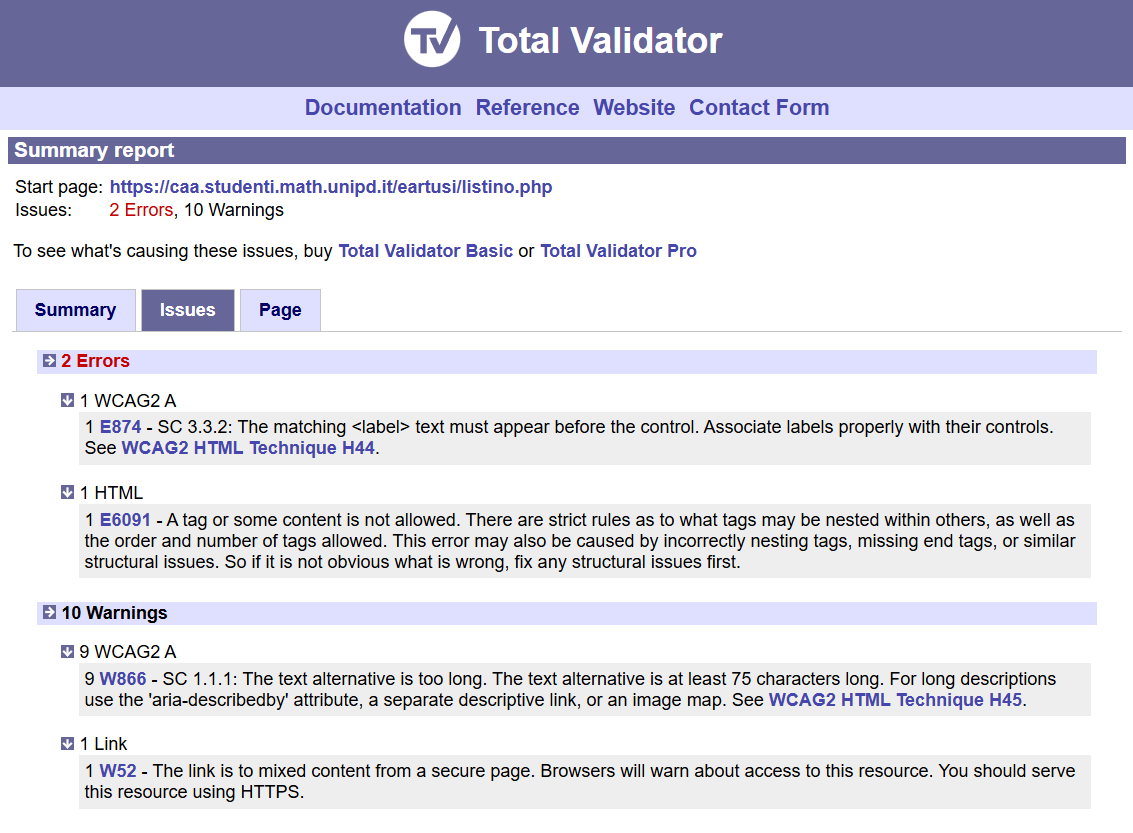
\includegraphics[width=0.8\linewidth, alt={Screenshot dell'analisi di Total Validator sul sito web LuzzAuto}]{img/TV_luzzauto.png}
    \caption{Analisi di Total Validator sul sito web \textit{LuzzAuto}}\label{fig:TV_luzzauto}
\end{figure}

\noindent Come visibile in figura \ref{fig:TV_luzzauto}, sono segnalati solamente alcuni "Warning". Non sono quindi presenti veri e propri errori di accessibilità.

\subsubsection{Lighthouse}
\noindent Il report generato dallo strumento Lighthouse ha restituito un punteggio di 100/100 nella sezione Accessibility, indicando che, secondo le metriche automatiche adottate, non sono stati rilevati errori o problematiche di conformità (vedi figura \ref{fig:Lighthouse_luzzauto}).
\begin{figure}[H]
    \centering
    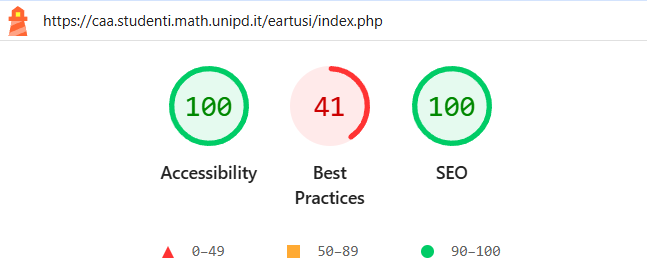
\includegraphics[width=0.6\linewidth, alt={Screenshot dell'analisi di Lighthouse sul sito web LuzzAuto}]{img/Lighthouse_luzzauto.png}
    \caption{Analisi di Lighthouse sul sito web \textit{LuzzAuto}}\label{fig:Lighthouse_luzzauto}
\end{figure}

\subsubsection{SviluppAbile}
\noindent Nella tabella \ref{tab:luzzauto} vengono riportati i risultati ottenuti utilizzando l'estensione \textit{SviluppAbile}.
\begin{footnotesize}
\begin{longtable}[c]{|C{4.6cm}|C{4.6cm}|C{4.6cm}|}
\caption{Tabella riassuntiva analisi \textit{LuzzAuto} tramite \textit{SviluppAbile}}
\label{tab:luzzauto}\\
\hline
\textbf{Errori trovati} & \textbf{Errori non trovati} & \textbf{Falsi positivi}\\
\hline
\endfirsthead
\multicolumn{3}{c}%
{{\bfseries Tabella \thetable\ -- continua dalla pagina precedente}} \\
\hline
\textbf{Errori trovati} & \textbf{Errori non trovati} & \textbf{Falsi positivi}\\
\hline
\endhead
\hline
\multicolumn{3}{r}{{ -- continua nella pagina successiva}} \\
\endfoot
\hline
\endlastfoot
 & 
\begin{itemize}
    \item Contrasto insufficiente link visitati/non
\end{itemize}
 & \begin{itemize}
    \item Tabindex non adeguato
\end{itemize}\\
\hhline{|=|=|=|} 
0 & 1 & 1 \\
\end{longtable}
\end{footnotesize}

\noindent L'F\textsubscript{1}-score calcolato è $F_{1}=0$, valore che indica prestazioni non soddisfacenti in questo caso specifico. 
Ciò evidenzia la necessità di ulteriori miglioramenti nell’identificazione degli errori, soprattutto per quanto riguarda i falsi positivi.


\section{Test ``Modalità guidata''}
\noindent Per effettuare i test utili a dimostrare l'efficacia di \textit{SviluppAbile}, ho creato una semplice pagina \acrshort{html} (vedi figura \ref{fig:pagina_test}).
\begin{figure}[H]
    \centering
    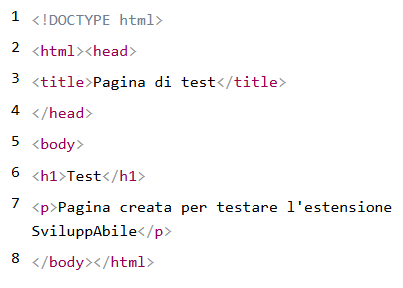
\includegraphics[width=0.5\linewidth, alt={Pagina \acrshort{html} base per effettuare i test della modalità guidata}]{img/test_MG.png}
    \caption{Pagina HTML base per effettuare i test della modalità guidata}\label{fig:pagina_test}
\end{figure}

\subsubsection*{\texttt{Come si crea un <head> che contenga tutti gli elementi utili per una pagina accessibile?}}
\begin{adjustwidth}{1cm}{1cm}
\noindent {\footnotesize Per creare un head accessibile, assicurati di includere i seguenti elementi:\\
1.  **Metatag Titolo (title)**: Utilizzato dal browser come titolo della finestra della pagina.\\
2.  **Metatag Descrizione (description)**: Descrive il contenuto della pagina e appare nella barra degli strumenti del browser e nei risultati dei motori di ricerca.\\
3.  **Metatag Chiave (keywords)**: Non più importante come in passato, ma puoi utilizzarla se necessario per le ricerche.\\
\\Inoltre, assicurati di utilizzare un markup semantico corretto per le sezioni della pagina. Ad esempio, puoi utilizzare `<header>`, `<nav>`, `<main>`, `<section>`, `<article>`, `footer>` in luogo di semplici div.\\
Infine, assicurati di aggiungere un elemento `alt` a tutte le immagini con una descrizione del contenuto dell'immagine.\\
\\CODICE SUGGERITO:\\
\texttt{1 <head>\\
2 <title>Pagina di test</title>\\
3 <meta charset="UTF-8">\\
4 <meta name="viewport" content="width=device-width, initial-scale=1.0">\\
5 <meta name="description" content="Pagina creata per testare l'estensione SviluppAbile">\\
6 <meta name="keywords" content="test,sviluppo accessibile">\\
7 </head>\\}}
\end{adjustwidth}


\subsubsection*{\texttt{Come posso ora creare dei paragrafi che rispettino le linee guida BEM?}}
\begin{adjustwidth}{1cm}{1cm}
\noindent {\footnotesize Per creare paragrafi in base alle linee guida BEM, puoi utilizzare la sintassi seguente:\\
1. Definisci un classico `.block\_\_element` per il contenuto del paragrafo: `class="block\_\_element"`\\
2. Utilizza `.block\_\_element--modificatore` per aggiungere modificatori: `class="block\_\_element --modificatore"`\\
In questo modo, i paragrafi saranno distinti e facili da identificare tramite la tecnica BEM.\\
\\Nota: Assicurati di sostituire `--modificatore` con il nome del modificatore effettivo nel tuo progetto.\\
\\CODICE SUGGERITO:\\
\texttt{1 <h1 class="block\_\_title">Titolo</h1>\\
2 <p class="block\_\_text --grande">Testo di esempio con un modificatore per il colore.</p>\\
3 <p class="block\_\_text --rosso">Testo di esempio con altro contenuto.</p>}\\
}
\end{adjustwidth}


\subsubsection*{\texttt{Come posso inserire immagini accessibili?}}
\begin{adjustwidth}{1cm}{1cm}
\noindent {\footnotesize Inserire immagini accessibili significa garantire che le informazioni contenute nelle immagini siano anche disponibili ai utenti con disabilità visiva. Ciò può essere fatto utilizzando l'attributo `alt` all'interno dell'elemento `<img>`.\\
In questo esempio, l'attributo `alt` contiene una descrizione breve e concisa della foto. Se il browser non è in grado di visualizzare l'immagine (ad esempio, se si utilizza un lettore schermo), la descrizione contenuta nell'attributo `alt` verrà visualizzata al posto dell'immagine.\\
Inoltre, per immagini decorative o grafici che non contengono informazioni importanti, è consigliabile utilizzare l'attributo `alt=""`, in modo da eliminare il testo alternativo dalla navigazione.\\
\\CODICE SUGGERITO:\\
\texttt{1 <img src="immagine.jpg" alt="Descrizione della foto">}
}
\end{adjustwidth}

\subsubsection*{\texttt{Come si crea una table rispettando le linee guida WCAG?}}
\begin{adjustwidth}{1cm}{1cm}
\noindent {\footnotesize Per creare una tabella accessibile secondo le linee guida WCAG, è importante fornire un'esperienza utente inclusiva e facilitare l'accessibilità a tutte le persone, in particolare alle persone con disabilità visive che utilizzano strumenti di lettura ad alta voce o tastiera. Ecco alcuni passaggi per creare una tabella accessibile:\\
1.  **Istruzioni per l'utilizzo della tabella**: fornire un'introduzione sulle informazioni presentate nella tabella e quali sono le colonne principali, aiutando gli utenti che utilizzano strumenti di lettura ad alta voce.\\
2.  **Tabella semantica con role="presentation" impostato su false**: questo ti permetterà a un assistente di lettura di comprendere il contenuto della tabella e fornirlo correttamente all'utente.\\
\\Nota che ogni elemento della tabella (celle, intestazioni) deve avere un id o un attributo aria-*, per fornire una descrizione dell'elemento e aiutare gli utenti con disabilità visive a comprendere il contenuto.\\
\\CODICE SUGGERITO:\\
\texttt{1 <table>\\
2 <caption>Esempio di tabella accessibile</caption>\\
3 <thead>\\
4 <tr role="row">\\
5 <th scope="col" id="nome">Nome</th>\\
6 <th scope="col" id="età">Età</th>\\
7 </tr>\\
8 </thead>\\
9 <tbody>\\
10 <tr role="row">\\
11 <td headers="nome">Mario Rossi</td>\\
12 <td headers="età">32 anni</td>\\
13 </tr>\\
14 <tr role="row">\\
15 <td headers="nome">Giovanni Bianchi</td>\\
16 <td headers="età">35 anni</td>\\
17 </tr>\\
18 </tbody>\\
19 </table>}
}
\end{adjustwidth}


\subsubsection*{\texttt{Come posso utilizzare gli attributi ARIA per migliorare l'accessibilità degli elementi interattivi?}}
\begin{adjustwidth}{1cm}{1cm}
\noindent {\footnotesize Gli attributi ARIA (Accessible Rich Internet Applications) sono stati sviluppati per rendere le applicazioni web accessibili a tutti, nonostante eventuali disabilità. Sono utilizzati per aggiungere funzionalità di navigazione e controllo agli elementi interattivi come i bottoni e gli elementi dropdown.\\
Per migliorare l'accessibilità degli elementi interattivi tramite ARIA, ti suggerisco di utilizzare le seguenti strategie:\\
1.  Utilizza il role di un elemento (ad esempio `button`, `menuitem`) per specificarne la funzione.\\
2.  Aggiungi gli attributi aria-label e aria-describedby per fornire una descrizione dell'elemento interattivo.\\
3.  Utilizza l'attributo aria-haspopup per indicare se un elemento è un menu o una lista.\\
\\In questo modo, l'elemento interattivo sarà più facile da navigare e controllare tramite strumenti assistivi come screen reader e mouse navigator.\\
Per ulteriori informazioni sugli attributi ARIA, ti consiglio di consultare la documentazione ufficiale dell'W3C.\\
\\CODICE SUGGERITO:\\
\texttt{1 <!DOCTYPE html>\\
2 <html><head>\\
3 <title>Pagina di test</title>\\
4 </head>\\
5 <body>\\
6 <!-- Utilizzo del role e degli attributi ARIA per il bottone -->\\
7 <button role="button" aria-label="Clicca per eseguire l'azione"> Esegui azione </button>\\
8 <!-- Utilizzo del role e degli attributi ARIA per il menu -->\\
9 <ul role="menu">\\
10 <li role="presentation">\\
11 <a href="\#" aria-label="Opzione 1" aria-haspopup="true">Opzione 1</a>\\
12 <ul role="sottomenu">\\
13 <li role="presentation"><a href="\#" aria-label="Sottopagina 1.1">Sottopagina 1.1</a></li>\\
14 <li role="presentation"><a href="\#" aria-label="Sottopagina 1.2">Sottopagina 1.2</a></li>\\
15 </ul></li></ul>\\
16 </body></html>}
}
\end{adjustwidth}
